\documentclass[12pt]{article}

% set margins according to Reimer's wishes
\usepackage[margin=1.0in]{geometry}

% nag if old commands or packages used
\usepackage{nag}

\usepackage{graphicx}
\usepackage{rotating}
\usepackage{float}
\usepackage{hyperref}
\usepackage{siunitx}
\usepackage{mhchem}
\usepackage{subfig}
\usepackage[final]{pdfpages}

\title{Simulation Summary}
\author{
        Henry Baxter \\
                Department of Physics and Astronomy\\
        University of Victoria\\
        henry.baxter@gmail.com
}
\date{\today}


\begin{document}
\maketitle

\section*{Abstract}

Dose simulations on a cylindrical water phantom were run for various hexagonal holed collimators using a 200keV electron gun with Tungsten reflection target as the X-ray source. Multiple row collimators were found to have a negative impact on both absolute dose delivered, and target to skin ratio. Septa widths down to 50 microns were found to provide sufficient collimation such that target to skin ratio was maintained, while increasing absolute dose delivered by almost 30\% (50 micron vs 500 micron). Convergent holed collimators are adequate for small lesion sizes, but do not provide coverage for larger lesions, though more investigation into alternative methods is required. Divergent holed collimators deliver more dose to the skin, but this also requires more thorough investigation.


\section*{Caveats}
Due to an important adjustment in skin dose calculation and the form of the phantom, the beam and arc weighting optimization is no longer calculating optimal treatments.  This distorts some of the imagery and dose results, however the results are still comparable against each other. Fixing this problem is not yet possible due to time constraints.


\section*{Simulation Properties}

Please examine Figure 1 to see the general geometry, the terminology, and the coordinate system used throughout. Note that the coordinate system on the dose contour plots in individual simulation reports has changed to conform to the coordinates of the rest of the report. The following figure was created in Sketchup, and the file is currently available at \url{https://s3-us-west-2.amazonaws.com/xcite-simulations/conceptual-diagram.skp}.

\begin{figure}[H]
\centering
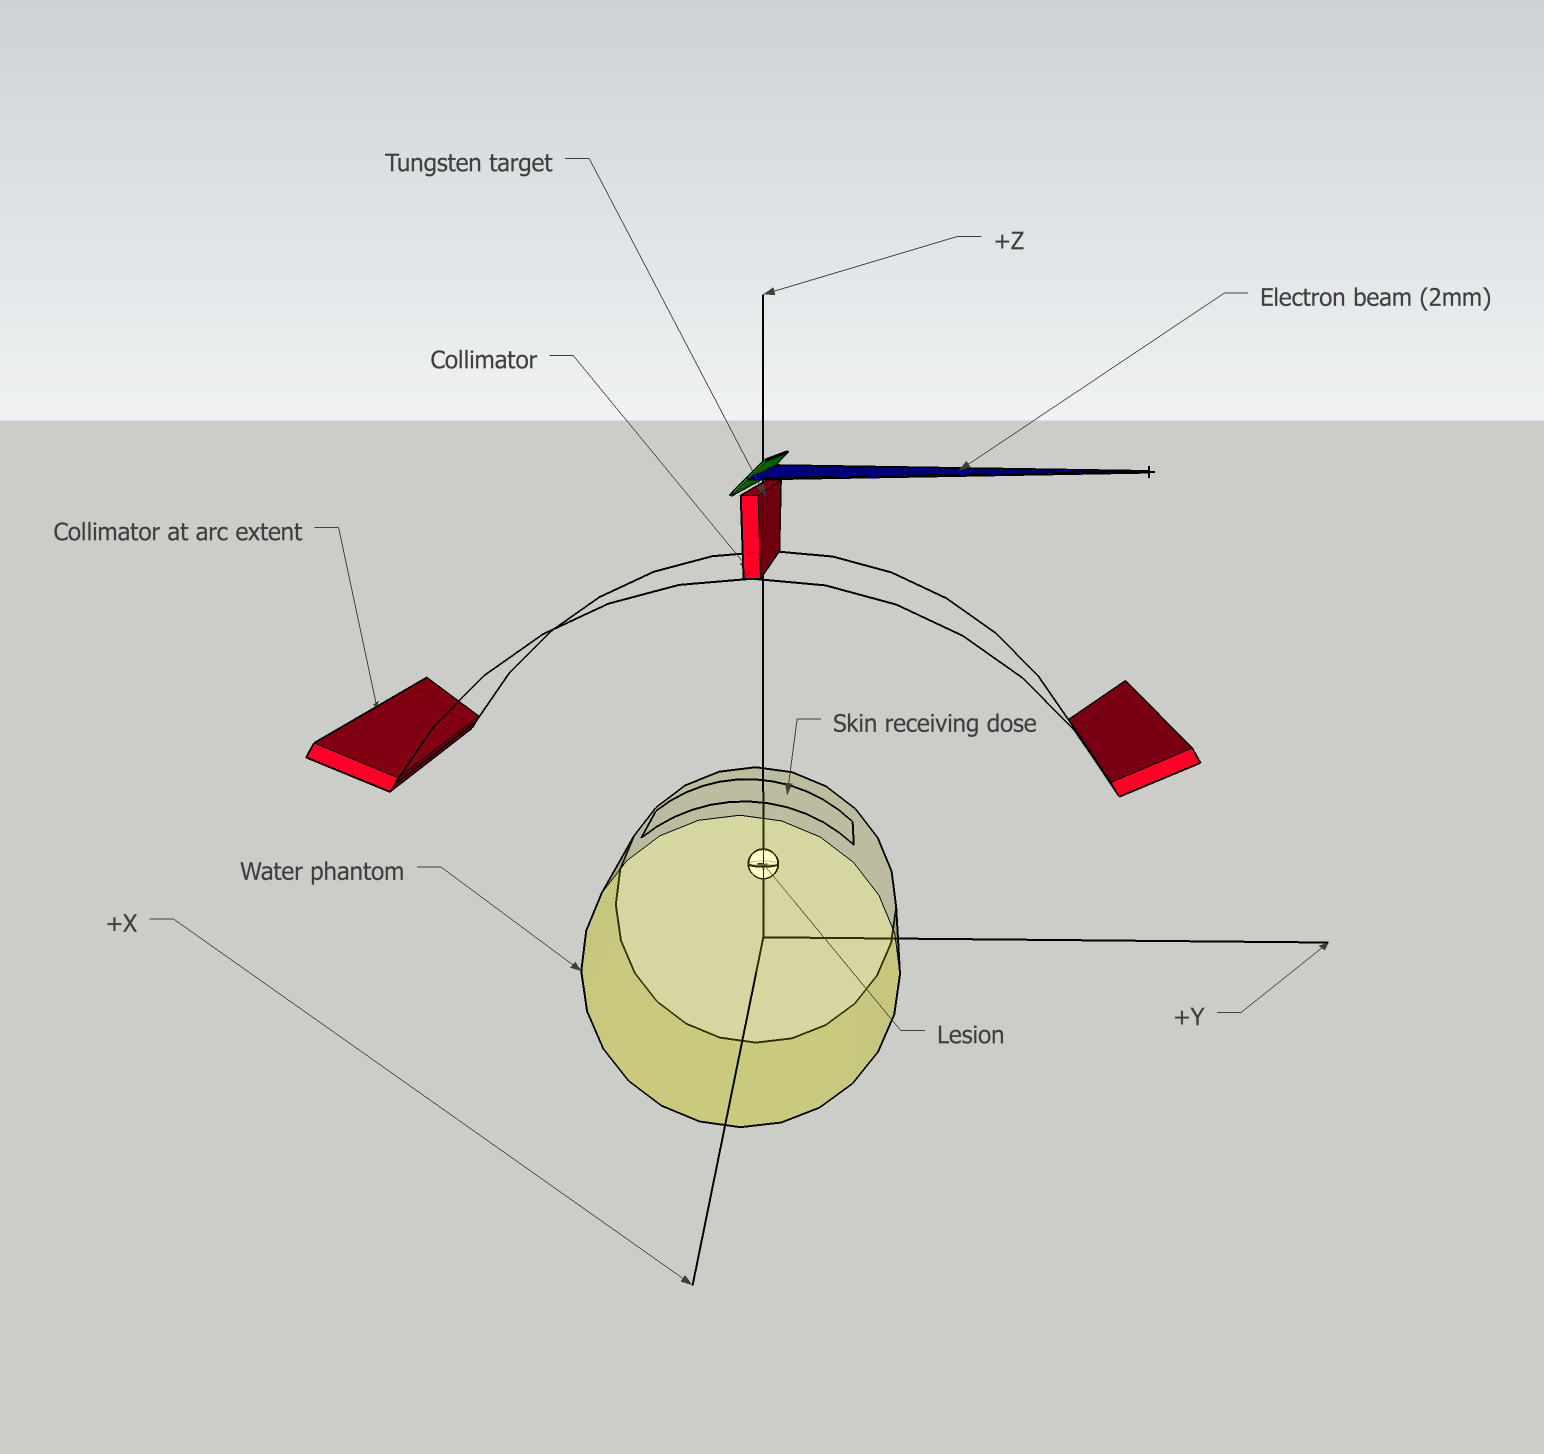
\includegraphics[scale=0.3]{../conceptual-diagram.png}
\caption{3D Model}
\end{figure}

\subsection*{Scanning Beam}
An electron scanning beam sweeping across a \SI{75.0}{\cm} Tungsten target was modelled. A total of 374 discrete beam \SI{0.2}{\cm} wide beamlets (x direction) were used to simulate the sweep, with beam incident positions $\SI{0.2}{\cm}$ apart. See Figure 2 for an idea of how this works. Note that the pink lines show the \SI{0.2}{\cm} distance between beamlet axes.

\begin{figure}[H]
\centering
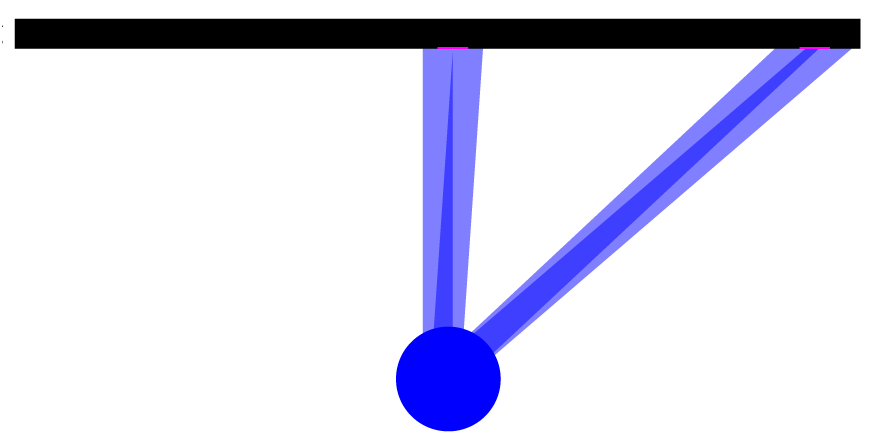
\includegraphics[scale=0.3]{../beam-geometry.png}
\caption{Electron Beam Overlap}
\end{figure}

Simulations used either a \SI{0.2}{\cm} or \SI{1.0}{\cm} beamlet height (z direction) to model a scanning beam of corresponding dimension. Each beamlet was a uniformly distributed rectangle.

\subsection*{Reflection Target and Filter}
The target and filter can be seen in Figure 3. The Tungsten target is the slender line (red) on the copper backing (green). The X-rays generated go through \SI{0.2}{\cm} of Aluminum, then \SI{0.3}{\cm} of water, and finally \SI{0.05}{\cm} of 304 Steel.

\begin{figure}[H]
\centering
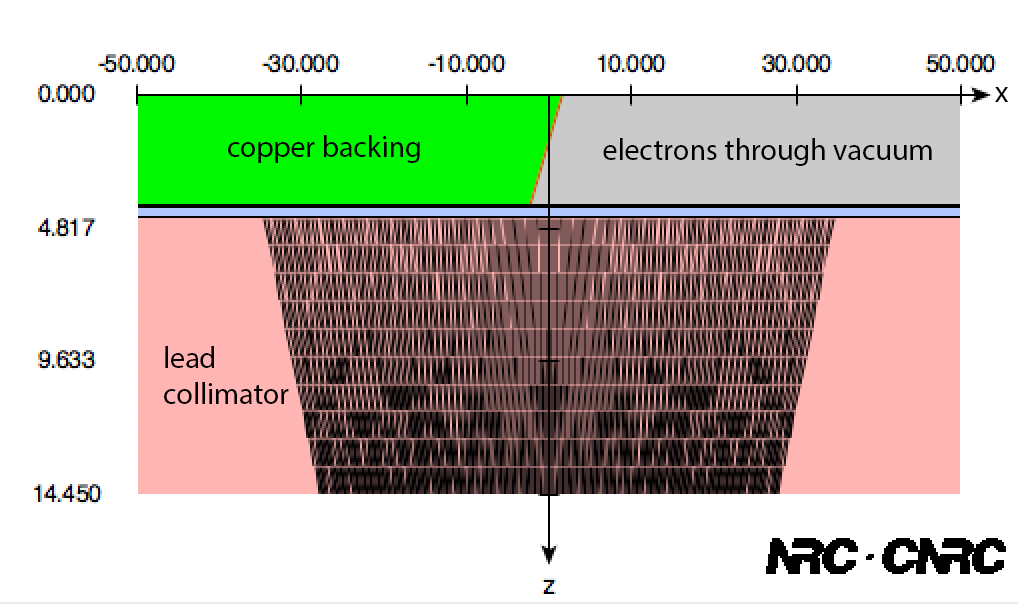
\includegraphics[scale=0.3]{../egs-geometry.png}
\caption{EGSnrc Target Dimensions}
\end{figure}

\subsection*{Collimator Design}
Collimators are modelled using a \SI{50.0}{\cm} by \SI{50.0}{\cm} by \SI{10.0}{\cm} block of lead that has hexagonal holes cut out of it. Visualizations of the collimator (the SCAD file referenced later) are provided as a negative space. That is, the holes (air) are solid objects, and everything else is assumed to be lead.

\begin{figure}[H]
\centering
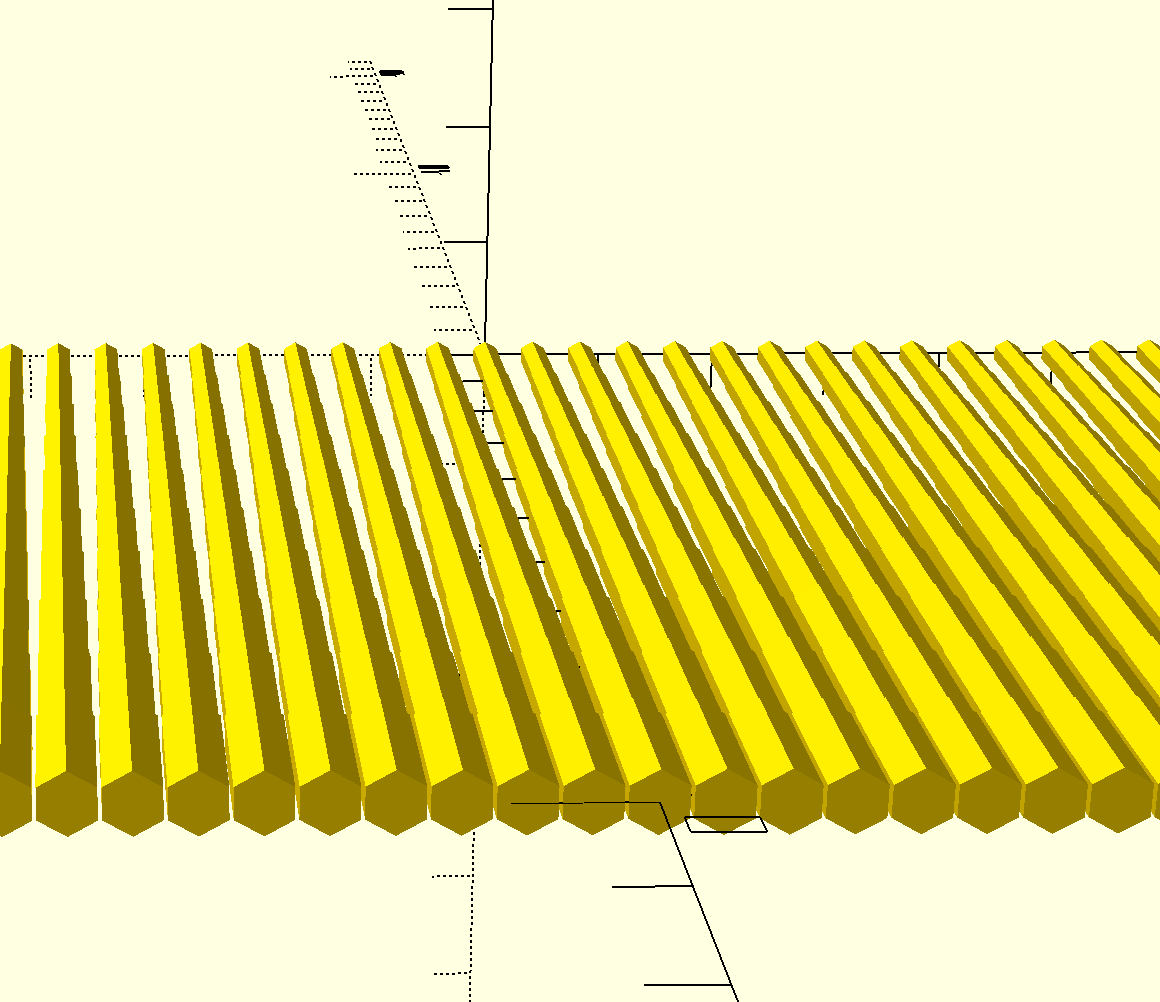
\includegraphics[scale=0.3]{../collimator.png}
\caption{Example SCAD Visualization}
\end{figure}

Manipulation of the SCAD files requires \url{http://www.openscad.org/}, and for an example consider viewing \url{https://s3-us-west-2.amazonaws.com/xcite-simulations/Converging-5-row-3mm/ collimator.scad}

\section*{Simulations}

\subsection*{Target to Skin}
Target to skin ratio is given by
\[
	TS = \frac{\mu_T}{\mu_S},
\]
where $\mu_T$ is the mean dose inside the lesion, and $\mu_S$ is the mean dose in the skin patch (see Figure 1). A larger value indicates the more favourable outcome.
\begin{table}[H]
\begin{tabular}{l l l l l}
	& Stationary & Weighted & Arc & Weighted Arc \\
	((* for s in simulations *))
	(((s.name))) & ((( s['results']['target_to_skin']['stationary']|f ))) & ((( s['results']['target_to_skin']['stationary-weighted']|f ))) & ((( s['results']['target_to_skin']['arc']|f ))) & ((( s['results']['target_to_skin']['arc-weighted']|f ))) \\
	((* endfor *))
\end{tabular}
\end{table}

\subsection*{Absolute Doses}
Dose is described in grays deposited in 30 minutes at 200 milliamps in the weighted arced treatment plan.

The absolute maximum and minimum doses inside the target volume are denoted by $D_{\mathrm{max}}$ and $D_{\mathrm{min}}$ respectively. The $D_n$ value is the minimum dose that $n\%$ of the target received. Concretely, $D_{90} = 1$ would indicate that 90\% of the target volume received \SI{1}{\gray} in 30 minutes, while 10\% received less than \SI{1}{\gray}.

Note that this implies $D_{\mathrm{min}} = D_{100}$.

\textbf{Unless otherwise indicated}, hexagonal holes have an in-diameter of \SI{2}{\mm} and septa widths are \SI{0.5}{\mm}.

\begin{table}[H]
\begin{tabular}{l l l l l l}
	& $D_{\mathrm{max}}$ & $D_{\mathrm{min}}$ & $D_{90}$ & $D_{95}$ & $D_{100}$ \\
	((* for s in simulations *))
	(((s.name))) & (((s['results']['doses']['absolute']['max']|f ))) & (((s['results']['doses']['absolute']['min']|f ))) & (((s['results']['doses']['absolute']['90']|f ))) & (((s['results']['doses']['absolute']['95']|f ))) & (((s['results']['doses']['absolute']['100']|f )))\\
	((* endfor *))
\end{tabular}
\end{table}

Simulations are of different collimators generating different distributions and numbers of particles, and every simulation models phantom voxels each with their own uncertainty based on this number and distribution. It is possible to come up with a rigorous error bound on each of the above values, but this has not been done due to time constraints. A conservative approximation is that these dose values are accurate to the nearest unit.

\subsection*{Raw results}
Each simulation generates a variety of files that are saved and can be made available, including dose distributions, phase space files, individual plot figures, and other intermediary information. The following are among the most useful: a pdf report that includes simulation parameters, plots, and a summary; a SCAD file with negative space geometry of the collimator itself; a TOML file that is the plain text input fed to the simulation process, along with some numerical results under the [results] heading.

For convenience, the Diverging 1cm Lesion report has been included in this report below the raw results listing.

\begin{itemize}
((* for s in simulations *))
	\item ((( s.name )))
\begin{itemize}
	((* for url in s.urls *))
	\item \url{((( url )))}
	((* endfor *))
\end{itemize}
((* endfor *))
\end{itemize}

\includepdf[pages=-]{../reports/Diverging-1cm-Lesion/Diverging-1cm-Lesion.pdf}

\end{document}

